\section{Related Work}
\label{relatedWorks}
\subsection{Natural Language Video Localization (NLVL)}
Previous works on NLVL can be categorized into proposal-based~\cite{liu_exploring_2022, gao_relation-aware_2021, soldan_vlg-net_2021, xiao_boundary_2021, yang_deconfounded_2021, gao_fast_2021, yu_intra-_2020, wu_learning_2022} and proposal-free approaches~\cite{rodriguez_proposal-free_2020, chen_hierarchical_2020, mun_local-global_2020, zeng_multi-modal_2021, zhao_cascaded_2021, zhang_natural_2022, rodriguez-opazo_dori_2021}. Proposal-based methods employ a generate-and-rank strategy, \ie generating candidate video moments and subsequently ranking them based on their alignment with the given textual query. In contrast, proposal-free methods directly regress on the untrimmed video, estimating the boundaries of the target video segment based on the query.

The majority of NLVL works are fully supervised, with proposal-free methods primarily focusing on segment localization or regression accuracy~\cite{zeng_dense_2020, wang_temporally_2020, rodriguez-opazo_dori_2021}, while proposal-based concentrating on improving the quality of the proposed video moment candidates~\cite{xiao_boundary_2021}. To effectively capture cross-modal relationships, several works transform either the video or query modalities, or both, into graphs and perform graph matching~\cite{soldan_vlg-net_2021, rodriguez-opazo_dori_2021, zeng_multi-modal_2021, chen_hierarchical_2020}. Some proposal-free works utilize convolutions to capture long-span dependencies within videos~\cite{li_proposal-free_2021} or as a form of cross-modal interaction~\cite{zhang_natural_2022, chen_hierarchical_2020}. Moreover, there exist works that reframe NLVL into a generative task~\cite{li2023momentdiff} or traditional NLP tasks such as multiple-choice reading comprehension~\cite{gao_relation-aware_2021} and dependency parsing~\cite{liu_context-aware_2021}. 

\subsection{Weakly-Supervised and Zero-shot NLVL Methods}
Fully supervised methods achieve impressive performance but require laborious
fine-grained video segment annotations corresponding to queries that are often prohibitively expensive for adapting to new domains. To address this challenge, weakly supervised methods have emerged, which operate with paired video-query data but without the need for precise video segment span annotations 
\cite{huang_cross-sentence_2021,zhang_counterfactual_2020,ma_vlanet_2020, 
detr}.
Many weakly-supervised approaches leverage contrastive learning to improve visual-textual alignment \cite{zhang_counterfactual_2020, zhang_video_2021, ma_vlanet_2020}. Recent work employs graph-based methodologies to capture contextual relationships between frames \cite{tan_logan_2021} and iterative approaches for fine-grained alignment between individual query tokens and video frames \cite{wang_fine-grained_2021}. 

\begin{figure*}[t!]
    \centering
    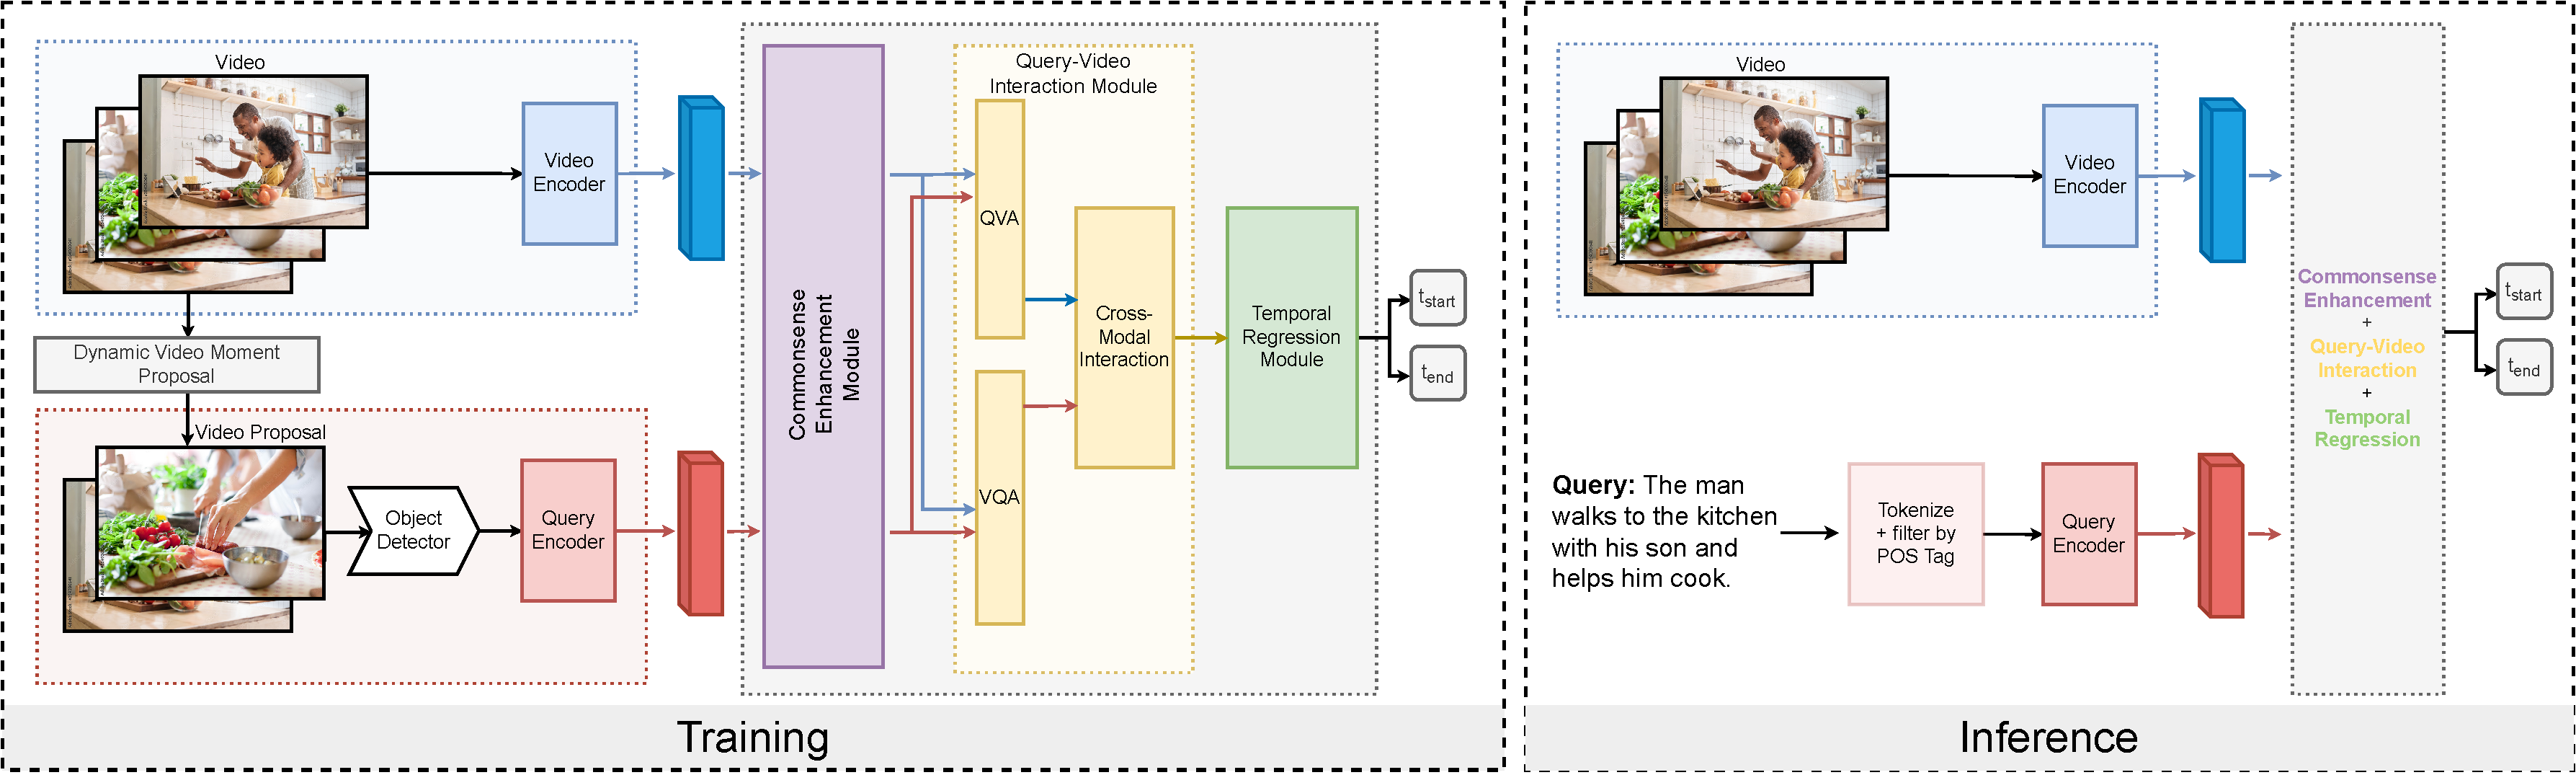
\includegraphics[width=0.95\textwidth]{figures/figure_files/ApproachFull.pdf}
    \caption{\modelname consists of a \textbf{\textcolor{Cerulean}{Video Encoder}} and a \textbf{\textcolor{Red}{Query Encoder}}, the proposed \textbf{\textcolor{RoyalPurple}{Commonsense Enhancement}}, \textbf{\textcolor{Golden}{Cross-modal (video-query) Interaction}}, and a \textbf{\textcolor{ForestGreen}{Temporal Regression}} module. During training, \modelname utilizes a Dynamic Video Moment Proposal module to extract a video moment span \(V_{\text{span}}\) and an off-the-shelf object detector to detect objects (nouns) in \(V_{\text{span}}\). During inference, the given natural language query is converted to a simplified query using a part-of-speech tagger. }
    \label{fig:approach}
\end{figure*}
Despite requiring fewer annotations, the effort involved in acquiring queries is still substantial. Unsupervised iterative approaches \cite{liu_unsupervised_2022} and zero-shot NLVL (ZS-NLVL) \cite{nam_zero-shot_2021} address this issue. ZS-NLVL aims to train an NLVL model using raw videos alone in a self-supervised setting, by generating video moments and corresponding pseudo-queries dynamically.
Pseudo-query generation is critical in zero-shot localization methods, although limited work has been done in this direction. \citet{nam_zero-shot_2021} introduce pseudo-query generation for video localization, and subsequently, \citet{jiang_pseudo-q_2022} for language grounding in images.
\citet{nam_zero-shot_2021} consider a pseudo-query to be an unordered list of nouns and verbs, obtained from an off-the-shelf object detector and a fine-tuned language model (LM) that predicts the most probable verbs conditioned on the nouns. While the objects are grounded in the video segment, the generation of verbs is not, potentially introducing irrelevant verbs and resulting in noisy pseudo-queries. Moreover, explicit verb-noun co-occurrences may encourage the localization model to learn spurious latent relationships and co-occurrence patterns between noun and verb data.
\citet{kim2023language} propose a language-free approach that leverages the aligned visual-language space of a pretrained CLIP model. A limitation is primarily relying on visual and temporal cues for video grounding but not fully capturing higher-level contextual knowledge and implicit relationships often conveyed through natural language. This could hinder the model's ability to understand and localize complex and nuanced events in videos that require additional context and reasoning beyond visual features.
In contrast, \modelname enriches the extracted video and pseudo-query features with commonsensical information. By considering spatiotemporal, causal, and physical relations w.r.t. the visual information, our model reasons beyond video cues and grounds pseudo-query information in the video.

\subsection{Commonsense in Video-Language Tasks}
Recent video-language research has shifted towards enhancing reasoning capabilities rather than solely focusing on recognition. Datasets such as Video2Commonsense \cite{fang_video2commonsense_2020}, Something Something \cite{goyal_something_2017}, Violin \cite{liu_violin_2020}, SUTD-TrafficQA \cite{peng_multi-modal_2021}, and VLEP \cite{lei_what_2020} emphasize commonsense reasoning. Metrics have also been proposed to evaluate the commonsense reasoning abilities of video-language models \cite{shin_cogme_2021,park_exposing_2022}. 
Commonsense has also been incorporated into tasks such as video captioning \cite{yu_hybrid_2021}, video question answering \cite{li_representation_2022}, and visual story generation \cite{maharana_integrating_2021}. 
Existing methods enhance query-based video retrieval using a co-occurrence graph of concepts mined from the target video moment \cite{wu_learning_2022,cao_visual_2022}. However, both are proposal-based fully supervised approaches that rely on fine-grained annotations and the quality of candidate video moments, let alone solely exploit the internal relations between the detected visual objects through a co-occurrence graph of entities as opposed to using external knowledge sources. In contrast, we utilize structured knowledge sources such as ConceptNet \cite{speer_conceptnet_2017} to encode commonsense information and leverage explicit relations spanning spatial, temporal, and physical aspects. This allows us to access information beyond what visual and textual cues can provide.
